\documentclass[11pt]{article}
\usepackage{fullpage,amsmath,mathtools, algorithm2e, forest}
\usepackage[mathletters]{ucs}
\usepackage{hyperref}
\usepackage[utf8x]{inputenc}
\usepackage{graphicx}
\usepackage{listings}
\usepackage{courier}

\lstset{basicstyle=\footnotesize\ttfamily,breaklines=true}
\lstset{frame=single}

\graphicspath{ {./images/} }
\title{COMP4107 - Assignment 4}
\author{Student Name: Yunkai Wang\\
\text{Student Number: 100968473}\\\\
Student Name: Jules Kuehn\\
\text{Student Number: 100661464}}
\date{Fall 2018}
\begin{document}
\maketitle

\begin{enumerate}
\item \textbf{Modification of the dataset loaded.}\\
We modified the files so that they are all loading the CIFAR-10 dataset:\\
\textit{from keras.datasets import cifar10}
\item \textbf{Changing the number of convolutional layers and sizes of max pooling layers. You must investigate 5 different model scenarios.}\\
The five model scenarios we investigated (as labelled in Figure 3) are described below.
Changing the max pooling layers to a larger size did not improve results, so those experiments are omitted here. Such a change reduces the size too drastically when we are starting from a small 32 x 32 image. We did however use a 4 x 4 average pooling layer in \textbf{Bon (No FC)}, inspired by more current research which eschews fully connected layers in favor of average pooling the last convolutional layer.\\
VGG-D is inspired by VGG-Net model D and is overkill for the 32x32 images. The Bonaccorso model is named after the author of the blog post which suggested using this layer configuration (https://www.bonaccorso.eu/2016/08/06/cifar-10-image-classification-with-keras-convnet/).\\
When reading the configurations below, assume ReLU activations on all layers unless otherwise indicated. Shape at end of each layer is (width, height, depth).
    \begin{enumerate}
        \item \textbf{cnn.py} (q1-original-cnn-model.py)
            \begin{itemize}
                \item Input (32, 32, 3)
                \item Convolution: 3 x 3 kernel, 1 x 1 stride, 32 features. (32, 32, 32)
                \item Max pooling: 2 x 2 window, 2 x 2 stride. (16, 16, 32)
                \item Dropout
                \item Fully connected (625)
                \item Dropout
                \item Output - softmax (10)
            \end{itemize}
        \item \textbf{LeNet} (q1-lenet-model.py)
            \begin{itemize}
                \item Input (32, 32, 3)
                \item Convolution: 5 x 5 kernel, 1 x 1 stride, 6 features. (32, 32, 6)
                \item Max pooling: 2 x 2 window, 2 x 2 stride. (16, 16, 6)
                \item Dropout
                \item Convolution: 5 x 5 kernel, 1 x 1 stride, 16 features. (16, 16, 16)
                \item Max pooling: 2 x 2 window, 2 x 2 stride. (8, 8, 16)
                \item Fully connected (120)
                \item Dropout
                \item Fully connected (84)
                \item Dropout
                \item Output - softmax (10)
            \end{itemize}
        \item \textbf{VGG-D 10 layer} (q1-vggnet-d-model.py)
            \begin{itemize}
                \item Input (32, 32, 3)
                \item Convolution: 3 x 3 kernel, 1 x 1 stride, 64 features. (32, 32, 64)
                \item Convolution: 3 x 3 kernel, 1 x 1 stride, 64 features. (32, 32, 64)
                \item Max pooling: 2 x 2 window, 2 x 2 stride. (16, 16, 64)
                \item Dropout
                \item Convolution: 3 x 3 kernel, 1 x 1 stride, 128 features. (16, 16, 128)
                \item Convolution: 3 x 3 kernel, 1 x 1 stride, 128 features. (16, 16, 128)
                \item Max pooling: 2 x 2 window, 2 x 2 stride. (8, 8, 128)
                \item Dropout
                \item Convolution: 3 x 3 kernel, 1 x 1 stride, 256 features. (8, 8, 256)
                \item Convolution: 3 x 3 kernel, 1 x 1 stride, 256 features. (8, 8, 256)
                \item Convolution: 3 x 3 kernel, 1 x 1 stride, 256 features. (8, 8, 256)
                \item Max pooling: 2 x 2 window, 2 x 2 stride. (4, 4, 256)
                \item Dropout
                \item Convolution: 3 x 3 kernel, 1 x 1 stride, 512 features. (4, 4, 512)
                \item Convolution: 3 x 3 kernel, 1 x 1 stride, 512 features. (4, 4, 512)
                \item Convolution: 3 x 3 kernel, 1 x 1 stride, 512 features. (4, 4, 512)
                \item Max pooling: 2 x 2 window, 2 x 2 stride. (2, 2, 512)
                \item Dropout
                \item Fully connected (1024)
                \item Dropout
                \item Fully connected (256)
                \item Dropout
                \item Output - softmax (10)
            \end{itemize}
        \item \textbf{Bon} (q1-bonaccorso-model.py)
            \begin{itemize}
                \item Input (32, 32, 3)
                \item Convolution: 3 x 3 kernel, 1 x 1 stride, 32 features. (32, 32, 32)
                \item Convolution: 3 x 3 kernel, 1 x 1 stride, 64 features. (32, 32, 64)
                \item Max pooling: 2 x 2 window, 2 x 2 stride. (16, 16, 64)
                \item Dropout
                \item Convolution: 3 x 3 kernel, 1 x 1 stride, 128 features. (16, 16, 128)
                \item Max pooling: 2 x 2 window, 2 x 2 stride. (8, 8, 128)
                \item Convolution: 3 x 3 kernel, 1 x 1 stride, 128 features. (8, 8, 128)
                \item Max pooling: 2 x 2 window, 2 x 2 stride. (4, 4, 128)
                \item Dropout
                \item Fully connected (1024)
                \item Dropout
                \item Output - softmax (10)
            \end{itemize}
        \item \textbf{Bon (No FC)} (q1-bonaccorso-noFC-extra\_conv.py)
            \begin{itemize}
                \item Input (32, 32, 3)
                \item Convolution: 3 x 3 kernel, 1 x 1 stride, 32 features. (32, 32, 32)
                \item Convolution: 3 x 3 kernel, 1 x 1 stride, 64 features. (32, 32, 64)
                \item Max pooling: 2 x 2 window, 2 x 2 stride. (16, 16, 64)
                \item Dropout
                \item Convolution: 3 x 3 kernel, 1 x 1 stride, 128 features. (16, 16, 128)
                \item Max pooling: 2 x 2 window, 2 x 2 stride. (8, 8, 128)
                \item Convolution: 3 x 3 kernel, 1 x 1 stride, 128 features. (8, 8, 128)
                \item Max pooling: 2 x 2 window, 2 x 2 stride. (4, 4, 128)
                \item Dropout
                \item Convolution: 3 x 3 kernel, 1 x 1 stride, 256 features. (4, 4, 256)
                \item Average pooling: 4 x 4 window, 4 x 4 stride. (1, 1, 256)
                \item Dropout
                \item Output - softmax (10)
            \end{itemize}
    \end{enumerate}
\item \textbf{Provide a PDF image of your computational graph. This must be captured from TensorBoard.}\\
In the code (q1-original-cnn-model\_tensorboard.py), we separated the model into several layers, so that the resulting computational graph looks nicer. When the session runs, the graph is captured by tensorboard. Figure 1 shows the result directly downloaded from TensorBoard.
\begin{figure}[h!]
    \centering
     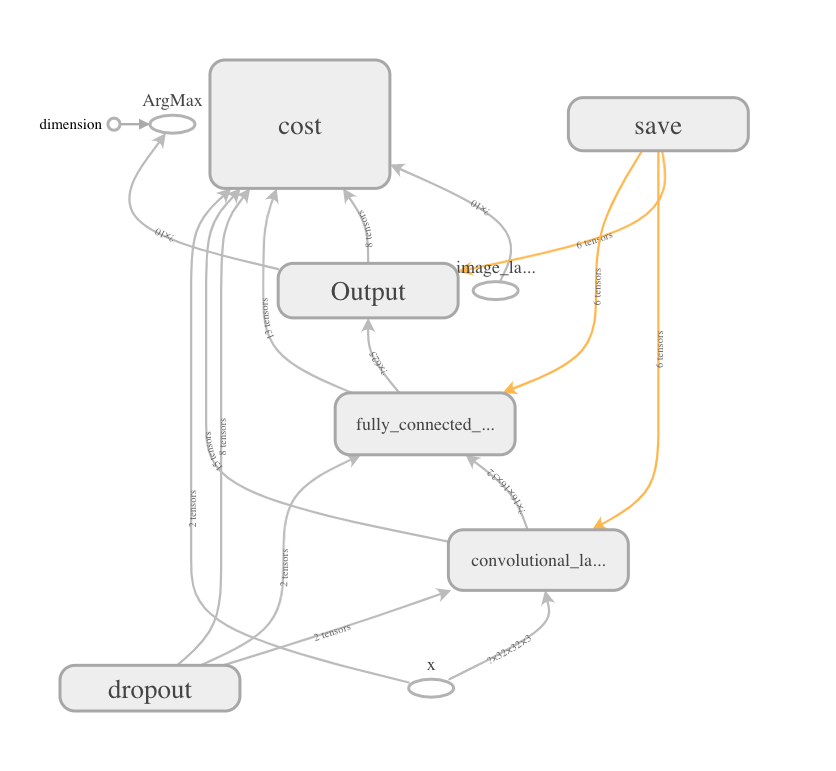
\includegraphics[width=0.5\textwidth]{images/computational_graph}
        \caption{Computational graph of the original CNN}
\end{figure}
Notice that since we group the variables by layers, so they are hidden inside those layers, but we include the generated event file, which can be used to launch the tensorboard (tensorboard --logdir=./tensorboard/original\_cnn/), and then the graph can be expanded there. For example, the max pooling layer is contained within convolutional\_layer shown in Figure 1.\\
We added the tensorboard code to the original model only, because doing the same for all other models is redundant, and the prof said that it is sufficient to include just one graph.
\item \textbf{Provide a capability to view weight histograms using TensorBoard. You must be able to checkpoint your model during training. See tutorial for details.}\\
Again, we made the change only in the q1-original-cnn-model\_tensorboard.py file. We saved our session after each epoch, which can be reflected at the bottom of the code. We created the following histograms (Figure 2) after training our model for 50 epochs.
\begin{figure}[h!]
    \centering
     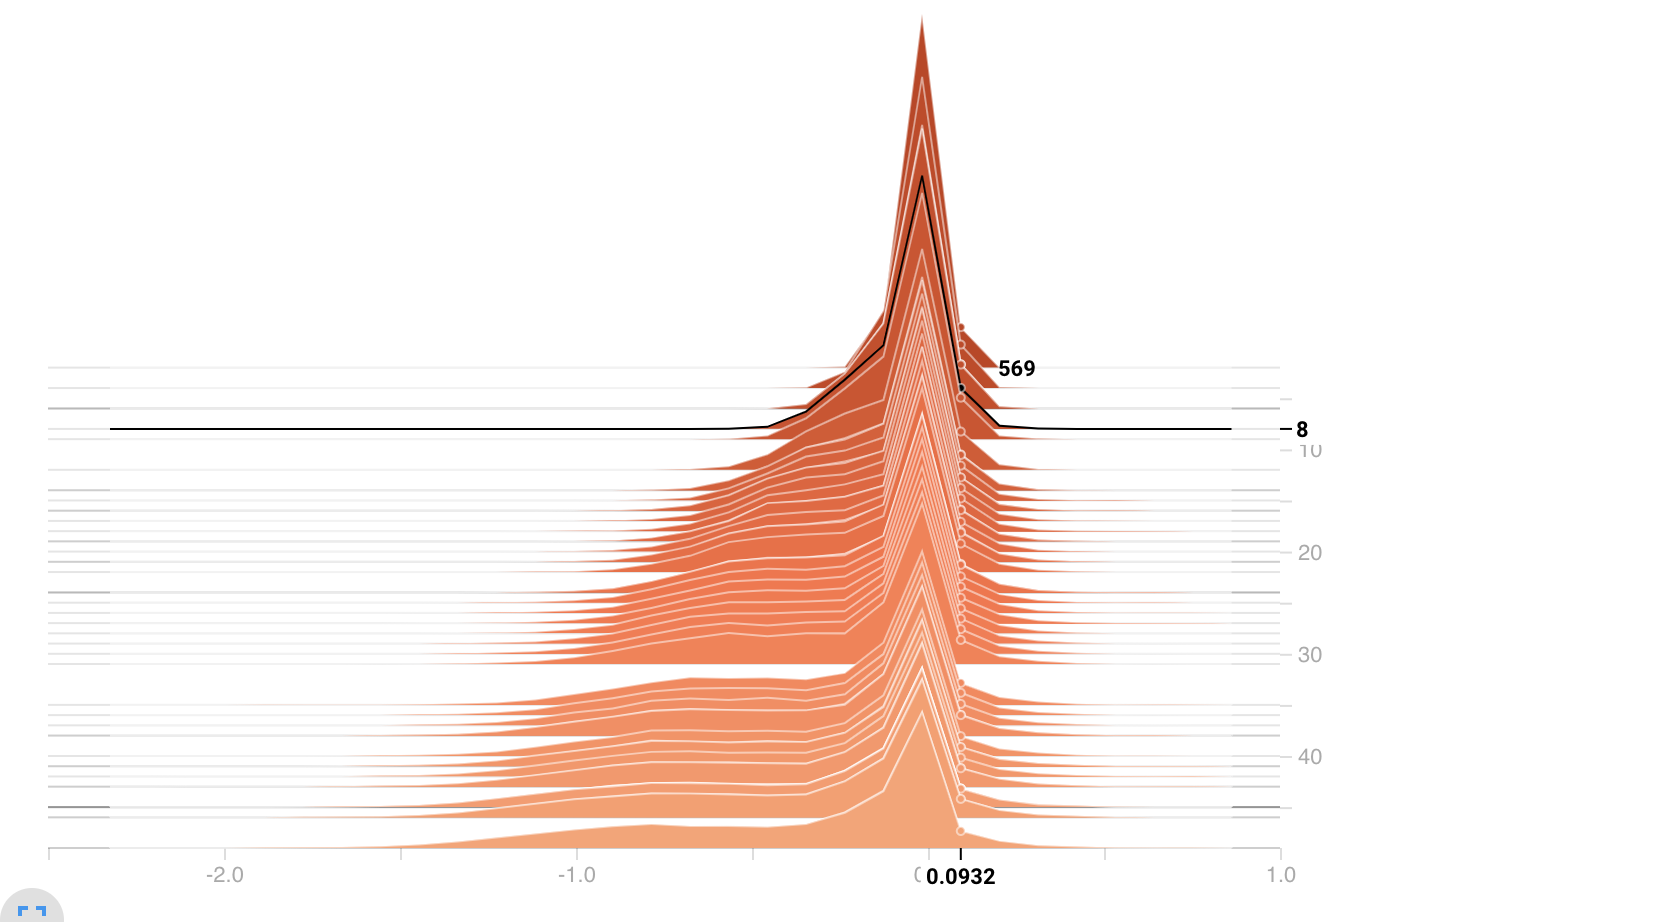
\includegraphics[width=0.5\textwidth]{images/histogram_1}
     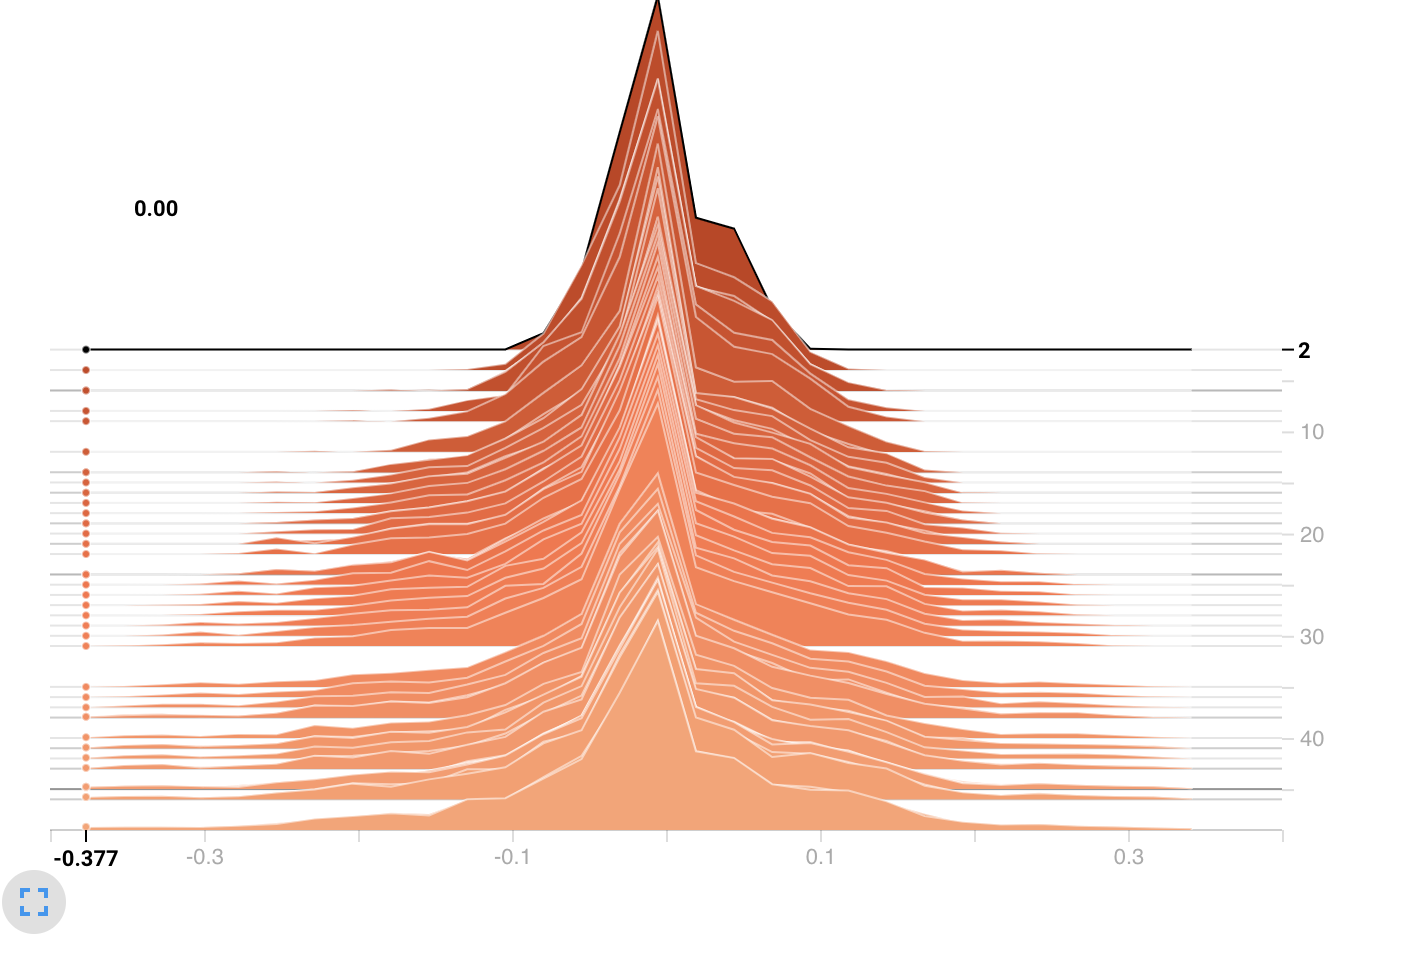
\includegraphics[width=0.5\textwidth]{images/histogram_2}
    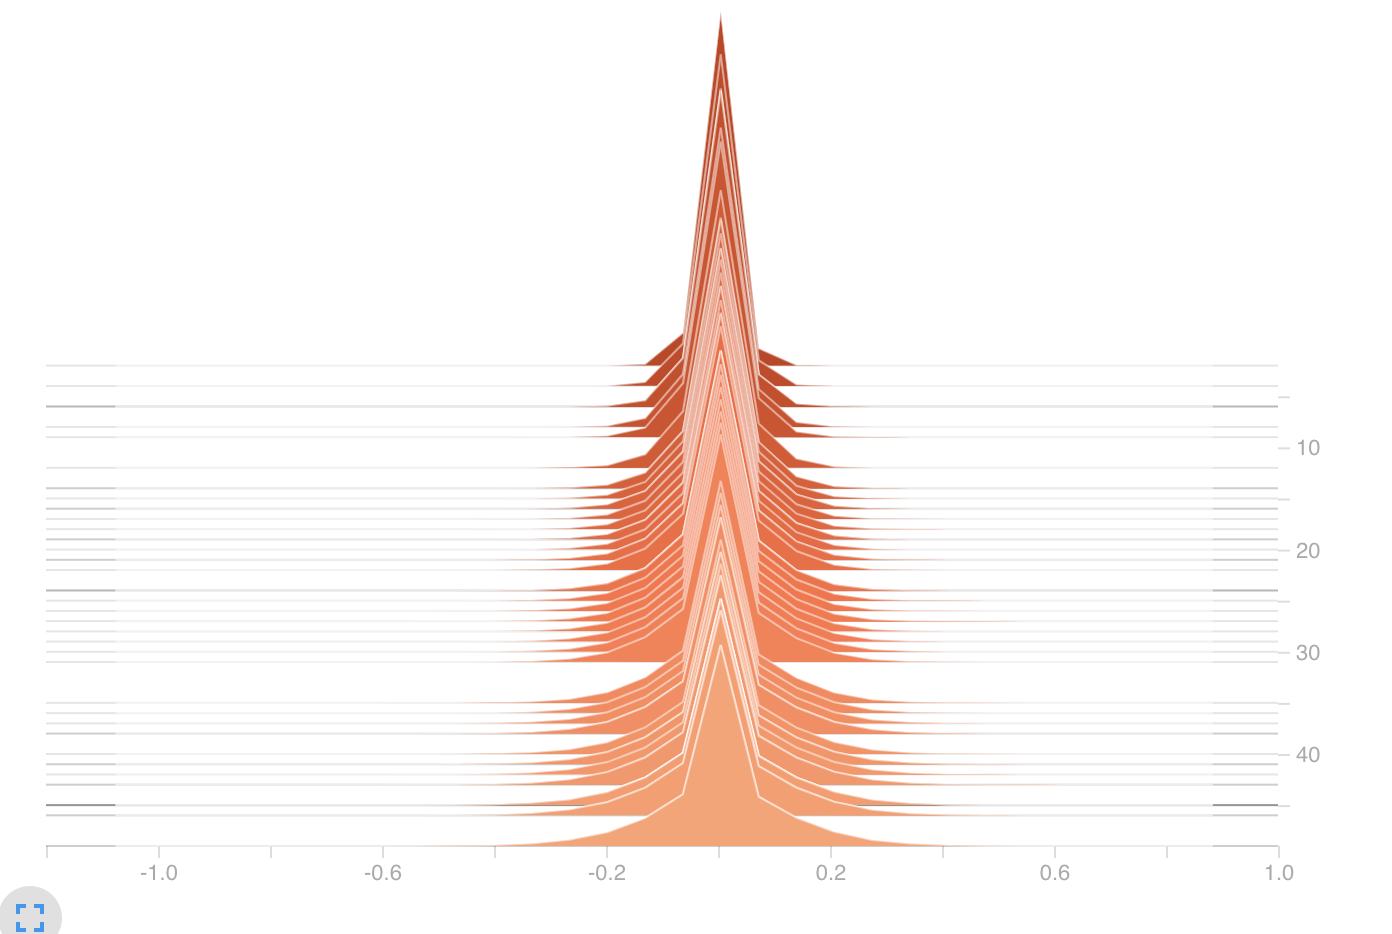
\includegraphics[width=0.5\textwidth]{images/histogram_3}
        \caption{Histograms of the weights in the model}
\end{figure}
\item \textbf{Provide a chart of the accuracy of your network for 1-15 epochs for the scenarios investigated.}\\
We trained all our 5 models for 50 epochs, and plotted the accuracies combined in one graph (Figure 3). We can see that the VGG-Net inspired network takes a long time to begin converging. This is likely due to the slow backpropagation through so many layers. The models taken from Bonaccorso achieve substantially better results than the rest. The best model uses no fully connected layers and achieving over 80\% accuracy.
\begin{figure}[h!]
    \centering
     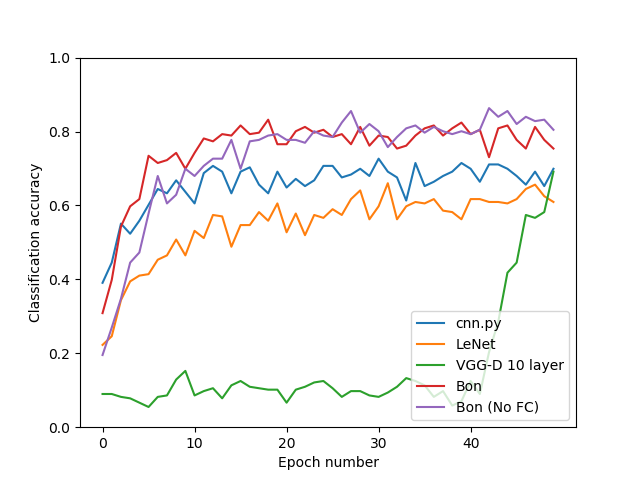
\includegraphics[width=0.75\textwidth]{images/accuracy}
        \caption{Accuracy of the CNNs}
\end{figure}
\item \textbf{Provide the capability to show the top 9 patches. Examples are shown on slides 63-65 of the CNN notes.}\\
The code to accomplish this task can be found in q1-bonaccorso-noFC-extra\_conv-model\_top9.py file. We run the session on layer 1, with a single image fed into the network as [X]. Then, we find the top 9 feature maps with highest activation (as determined by summing all pixels for each returned feature map). These feature maps are shown in Figure 4, along with the input images.
\begin{figure}[h!]
    \centering
     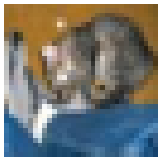
\includegraphics[width=0.25\textwidth]{images/0_input_image}
     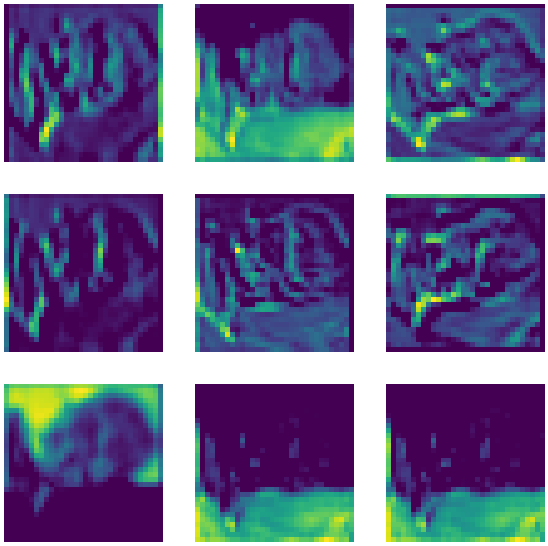
\includegraphics[width=0.25\textwidth]{images/0_top_layers}\\
     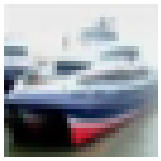
\includegraphics[width=0.25\textwidth]{images/1_input_image}
     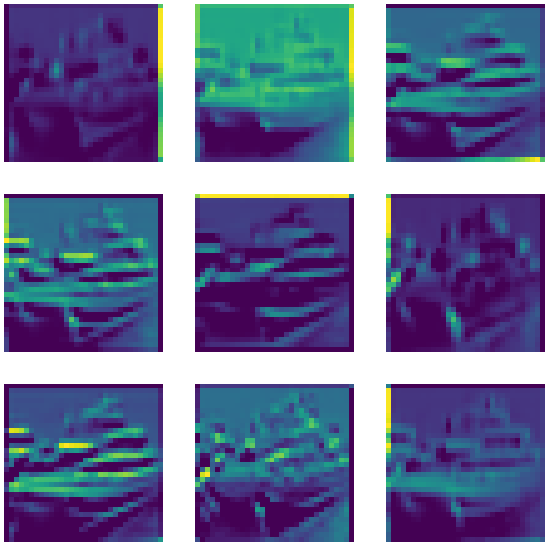
\includegraphics[width=0.25\textwidth]{images/1_top_layers}\\
     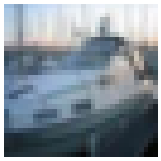
\includegraphics[width=0.25\textwidth]{images/2_input_image}
     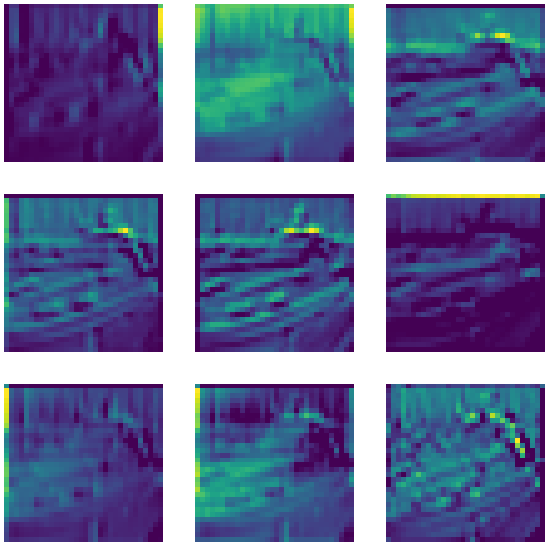
\includegraphics[width=0.25\textwidth]{images/2_top_layers}
        \caption{Top 9 activated features for a given image (Layer 1)}
\end{figure}

\end{enumerate}

\end{document}